% This is a latex template for an informal report with no title page, resembling 
% in format article manuscripts submitted to journals in political science or economics. 
% It is intended for use with documents derived from the R markdown template informal-report.Rmd. 
% It is heavily indebted to Steven Miller's article template at 
% https://github.com/svmiller/svm-r-markdown-templates, but 
% has accumulated various changes (sometimes enhancements) as I've used it. It is free for 
% anyone's use under the terms of the MIT license; see LICENSE.md. 


\documentclass[
  11pt,
  american,
  letterpaper,
  ]{article}
  

  \usepackage[margin=2.54cm]{geometry}
 
% \usepackage{textcomp}     % obsolete

\usepackage[usenames,dvipsnames,svgnames]{xcolor}   % all the colors, yes all of them

  \usepackage{graphicx,grffile}
  \makeatletter
  \def\maxwidth{\ifdim\Gin@nat@width>\linewidth\linewidth\else\Gin@nat@width\fi}
  \def\maxheight{\ifdim\Gin@nat@height>\textheight\textheight\else\Gin@nat@height\fi}
  \makeatother
  % Scale images if necessary, so that they will not overflow the page
  % margins by default, and it is still possible to overwrite the defaults
  % using explicit options in \includegraphics[width, height, ...]{}
  \setkeys{Gin}{width=\maxwidth,height=\maxheight,keepaspectratio}

\usepackage{ifxetex,ifluatex}

\ifxetex
  \usepackage{mathspec}
\else
  \usepackage{fontspec}
\fi

\defaultfontfeatures{Ligatures=TeX}

\usepackage{amssymb,amsmath}

\usepackage{microtype}
\usepackage{hyphenat}   % Use, for example, in government\hyp{}wide to prevent overfull hboxes
                        % \hyp{} provides the hyphen for hyphenated words while allowing 
                        % LaTeX to hyphenate the rest of the word if necessary. 

% use upquote if available, for straight quotes in verbatim environments
\IfFileExists{upquote.sty}{\usepackage{upquote}}{}

%% Fonts can be specified as fontfamily (e.g., "mathpazo" or "pagella" or using 
%% \setmainfont. Doing both wouldn't make sense, but after either, we allow defining 
%% specific fonts such as titlefont, authorfont, pagefont as exceptions. 

  \usepackage[]{mathpazo}
  %  % default selector: rm, sf, or tt
    \renewcommand{\familydefault}{\rmdefault}
  

  % no mainfont specified; default behavior specified differently
  
    \newcommand{\titlefont}{\normalfont}
  
    % font for author name on first page
    \newfontfamily\authorfont[]{zhv-Bol.otf}
  
  
    \newcommand{\pagefont}{\normalfont}
  
  
    \newcommand{\footnotefont}{\normalfont}
  
  
    \newcommand{\bibliofont}{\normalfont}
  

 
      \newcommand{\footnotefamily}{\rmfamily}
  

  % bibliography font size
  \newcommand{\bibliosize}{\footnotesize}



\usepackage[T1]{fontenc}
%% \usepackage[utf8]{inputenc} %% Not needed since xelatex uses utf8 natively

\usepackage[usenames,dvipsnames,svgnames]{xcolor}

      \setcounter{secnumdepth}{3}
  
\usepackage{abstract}
\renewcommand{\abstractname}{}    % clear the title
\renewcommand{\absnamepos}{empty} % originally center

\renewenvironment{abstract}
 {{%
    \setlength{\leftmargin}{0mm}%
    \setlength{\rightmargin}{\leftmargin}%
  }%
  \relax}%
 {\endlist}

\makeatletter
\def\@maketitle{%
  \newpage%
    {\titlefont\fontsize{18}{20}\selectfont\raggedright\setlength{\parindent}{0pt} \@title\par}%
}
\makeatother






  \title{ Report that I
wrote%  % extra %s to ensure no new paragraph before thanks
  %
    \thanks{\textbf{Corresponding author}:
\href{mailto:name@example.org}{\nolinkurl{name@example.org}}} 
   }
 

  \author{
      {Some Person}%
%    
      {}%
%    
      {Someone Else}%
%    
      {}}

\date{}
%%%%%%%%%%%%%%%%%%%%%%%%%%%%%%%%%%%%%%%%%%%%%%%%%%%%%%%%%%%%%%%%%%%%%%%%%%%%%%%%%
\usepackage{titlesec}
\titleformat*{\section}{\large\bfseries}
\titleformat*{\subsection}{\normalsize\bfseries}
\titleformat*{\subsubsection}{\normalsize\itshape}
\titleformat*{\paragraph}{\normalsize\itshape}
\titleformat*{\subparagraph}{\normalsize}

      \newcommand*{\supersectsize}{\Large}
        \newcommand*{\supersectseries}{\bfseries}
    \newcommand*{\supersection}[1]{{\noindent\supersectsize\supersectseries #1}}


\usepackage{tabu}

%% Page headers and footers

\usepackage{fancyhdr}
\pagestyle{fancy}

\setlength{\headheight}{13.6pt}

\fancyhf{} % clear all header and footer fields
\fancyfoot[C]{\pagefont\selectfont{\thepage}} % except the center
\fancyhead[C]{%
    %% For markings such as "DRAFT", "CONFIDENTIAL", ...
    {\sffamily\large%
      \color{ForestGreen}%
      \textbf{DRAFT}}%
  }
\renewcommand{\headrulewidth}{0pt}
\renewcommand{\footrulewidth}{0pt}

%% We want the same formatting if pagestyle gets set back to plain
\fancypagestyle{plain}{%
\fancyhf{} % clear all header and footer fields
\fancyfoot[C]{\pagefont\selectfont{\thepage}} % except the center
\fancyhead[C]{%
      {\sffamily\large%
      \color{ForestGreen}%
      \textbf{DRAFT}}%
  }
\renewcommand{\headrulewidth}{0pt}
\renewcommand{\footrulewidth}{0pt}}



\newtheorem{hypothesis}{Hypothesis}
\usepackage{setspace}

% Customize bullets: %{\textopenbullet} %{\rhd} %{\textbullet} 
  \renewcommand{\labelitemi}{\triangleright} 
  \renewcommand{\labelitemii}{\guillemotright} 
  \renewcommand{\labelitemiii}{\textbullet} 
  \renewcommand{\labelitemiv}{\textopenbullet} 

%% footnotes

% bottom option keeps footnotes from being rendered above bottom-of-page floats. 
% multiple option should place commas between footnote marks in adjacent locations; 
% seems not to be working. 
\usepackage[bottom,multiple]{footmisc}
\renewcommand\multfootsep{,}

% Force footnotes to be rendered with the specified footnote font or a correct 
% default font (not lmodern)
\let\oldfootnotelayout\footnotelayout
\renewcommand{\footnotelayout}{\oldfootnotelayout\footnotefont}

\usepackage{etoolbox} % we patch some internal footnote commands to get 
\makeatletter         % control over footnote fonts. 
\patchcmd{\@footnotetext}{\footnotesize}{\footnotefamily\footnotesize}{}{}
\patchcmd{\@makefnmark}{\normalfont}{\normalfont\footnotefamily\scriptsize}{}{}
\makeatother

\newcommand\blfootnote[1]{%   % for unnumbered footnotes: https://tex.stackexchange.com/a/30726/221633
  \begingroup
  \renewcommand\thefootnote{}\footnote{#1}%
  \addtocounter{footnote}{-1}%
  \endgroup
}

  \AtBeginEnvironment{quote}{\normalsize}
% \AtBeginEnvironment{quote}{\singlespace\vspace{-\topsep}\small}
% \AtEndEnvironment{quote}{\vspace{-\topsep}\endsinglespace}


      \usepackage{chngcntr}
    \counterwithin{figure}{section}
    \counterwithin{table}{section}
  

  \usepackage[toc]{appendix}

  \newcommand{\startofappendices}{
    \clearpage
    \pagebreak
    \begin{appendices}
          \renewcommand{\appendixname}{Appendix}
        \appendix
    \appendixpage
  }

  \newcommand{\appendicesendhere}{
    \clearpage
    \end{appendices}
    \renewcommand{\appendixname}{}
    \renewcommand{\appendixtocname}{}
  }

  \newcommand{\anappendix}[1]{
    \ifnum \value{section}>1
      \clearpage
      \pagebreak
      \setcounter{page}{1}
    \fi
      \pagenumbering{arabic}%
              \renewcommand{\thepage}{\thesection--\arabic{page}}%
          \section{#1} \label{Appendix \thesection}%
  }

% Set style of Appendices heading
  \renewcommand*{\appendixpagename}{\supersection{Appendices}}


  \usepackage [style=alphabetic]{biblatex}
  \renewcommand*{\bibfont}{\bibliofont\bibliosize\selectfont}
      \ExecuteBibliographyOptions{hyperref=true,backref=true}
        \addbibresource{generic.bib}
  

\newcommand{\startofreferences}{
  %\pagebreak
  \setcounter{secnumdepth}{0}
  \setcounter{page}{1}
      \pagenumbering{roman}
          \newcommand{\refpagenumberprefix}{ref--}
      \renewcommand{\thepage}{\refpagenumberprefix%
        \roman{page}}
      }

% Set style of References heading
\defbibheading{bibliography}[References]{\supersection{#1}\vspace{0.3cm}}


\usepackage{sparklines}
% The height of the sparklines in ex units
\renewcommand\sparklineheight{1.75}
% The line width
\setlength\sparklinethickness{0.4pt}
% The color of the sparkline
\definecolor{sparklinecolor}{named}{blue}
% The color of the sparkine rectangle when present
\definecolor{sparkrectanglecolor}{gray}{0.8}
% The dot width
\setlength\sparkdotwidth{2pt}
% The color of the spikes
\definecolor{sparkspikecolor}{named}{blue}
% The color of the bottom line when present
\definecolor{bottomlinecolor}{gray}{0.2}
% The thickness of the bottom line
\setlength\sparkbottomlinethickness{.1pt}
% The clipping separation (need sparklines v1.7 or later)
\setlength\sparklineclipsep{1pt}

%\usepackage{setspace}
\usepackage [american]{babel}
\usepackage [autostyle, english = american, maxlevel = 4]{csquotes}
\MakeOuterQuote{"}


  \renewcommand\textfraction{0.15}
  \usepackage{flafter}
  \usepackage[parfill]{parskip}
  \usepackage{booktabs}
  \usepackage{longtable}
  \usepackage{array}
  \usepackage{multirow}
  \usepackage{wrapfig}
  \usepackage{float}
  \usepackage{colortbl}
  \usepackage{pdflscape}
  \usepackage{tabu}
  \usepackage{threeparttable}
  \usepackage{threeparttablex}
  \usepackage[normalem]{ulem}
  \usepackage{makecell}
  \usepackage{xcolor}
  \usepackage{siunitx}

\usepackage{tabto}
\usepackage{float}
\usepackage{framed}

% This should regulate where figures float
% See: https://tex.stackexchange.com/questions/2275/keeping-tables-figures-close-to-where-they-are-mentioned
\usepackage[section]{placeins}  % also gives us \FloatBarrier

\usepackage{pgf}
\usepackage{verbatim}
\usepackage{environ}
\usepackage{pdfpages}  % include other pdf file using \includepdf[pages={-}]{filepath.pdf}
\usepackage{tcolorbox}

% move the hyperref stuff down here, after header-includes, to allow for - \usepackage{hyperref}

\makeatletter
\@ifpackageloaded{hyperref}
  {}
  {%
  \ifxetex
    \PassOptionsToPackage{hyphens}{url}
    \usepackage[setpagesize=false, % page size defined by xetex
                unicode=false, % unicode breaks when used with xetex
                xetex]{hyperref}
  \else
    \PassOptionsToPackage{hyphens}{url}
    \usepackage[unicode=true]{hyperref}
  \fi
}


\makeatother
\hypersetup{breaklinks=true,
            final=true,
            debug=true,
            pdfauthor={Some Person () and  (Sort of a
company) and Someone Else () and  (This PlaceThat Place)},
            pdfkeywords = {},  
            pdftitle={Report that I wrote},
                          colorlinks,
              citecolor=PineGreen,
              urlcolor=RoyalPurple,
              linkcolor=Maroon,
                        pdfborder={0 0 0}}
  
\urlstyle{sf}  % sans serif
% Add an option for endnotes. -----


% add tightlist ----------
\providecommand{\tightlist}{%
\setlength{\itemsep}{0pt}\setlength{\parskip}{0pt}}

% add some other packages ----------

% \usepackage{multicol}

% set default figure placement to htbp
\makeatletter
  \def\fps@figure{htbp}
\makeatother

\usepackage[labelfont=bf,%
textfont=normal,%
justification=justified,singlelinecheck=false]{caption}
% 
% \captionsetup[figure]{labelfont=it}



\begin{document}  %%%%%%%%%%%%%%%%%%%%%%%%%%%%%%%%%%%%%%%%%%%%%%%%%%%%%%%%%%%%%%

\pagenumbering{arabic}% resets `page` counter to 1 

    {%
    \setlength{\parindent}{0pt}
    \thispagestyle{plain}
    {\fontsize{18}{20}\selectfont\raggedright 
      \maketitle 
    }%
    {
      \vskip 13.5pt\relax \normalsize\fontsize{11}{13} 
      
        %
          \textbf{\authorfont Some Person}%
          %
        %
          \textbf{\authorfont }%
          \tabto{4.5cm}\emph{Sort of a company}\\%
        %
          \textbf{\authorfont Someone Else}%
          %
        %
          \textbf{\authorfont }%
          \tabto{4.5cm}\emph{This Place}\\\tabto{4.5cm}\emph{That
Place}\\%
        %
        \vskip -12.75pt % 2020-08-01
      %
    }%
  }%
  
      \begin{abstract}
    \hbox{\vrule height .2pt width \textwidth}%
          \vskip 2pt
        \noindent This is an R markdown template for an informal report
with no title page, resembling in format article manuscripts submitted
to journals in political science or economics. It is intended for use
with the corresponding latex template informal-report-template.tex. It
is heavily indebted to Steven Miller's article template at
\url{https://github.com/svmiller/svm-r-markdown-templates}, but has
accumulated various changes (sometimes enhancements) as I've used it. It
is free for anyone's use under the terms of the MIT license; see
LICENSE.md.
          \par
      \hbox{\vrule height .2pt width \textwidth}
        \end{abstract}
    \vskip -26.5pt
   % removetitleabstract

\noindent 
  

\blfootnote{\textbf{Current version:} September 03, 2021; \textbf{commit:} a12f71db 2021-04-23 UF! UC!}

\hypertarget{introduction}{%
\section{Introduction}\label{introduction}}

Lorem ipsum dolor sit amet, consectetur adipiscing elit, sed do eiusmod
tempor incididunt ut labore et dolore magna aliqua. Lorem ipsum dolor
sit amet, consectetur adipiscing elit, sed do eiusmod tempor incididunt
ut labore et dolore magna aliqua.Lorem ipsum dolor sit amet, consectetur
adipiscing elit, sed do eiusmod tempor incididunt ut labore et dolore
magna
aliqua.\autocite{nyserdaNewYorkState2019}\autocite{epaInventoryGreenhouseGas2017}
Lorem ipsum dolor sit amet, consectetur adipiscing elit, sed do eiusmod
tempor incididunt ut labore et dolore magna aliqua.

\begin{quote}
Lorem ipsum dolor sit amet, consectetur adipiscing elit, sed do eiusmod
tempor incididunt ut labore et dolore magna aliqua. Lorem ipsum dolor
sit amet, consectetur adipiscing elit, sed do eiusmod tempor incididunt
ut labore et dolore magna aliqua. Lorem ipsum dolor sit amet,
consectetur adipiscing elit, sed do eiusmod tempor incididunt ut labore
et dolore magna aliqua.
\end{quote}

\textit{This should be italicized.} \texttt{This should be monotype.}

\begin{itemize}
\tightlist
\item
  We have bullets

  \begin{itemize}
  \tightlist
  \item
    Yes we do

    \begin{itemize}
    \tightlist
    \item
      We have bullets

      \begin{itemize}
      \tightlist
      \item
        How 'bout you?
      \end{itemize}
    \end{itemize}
  \end{itemize}
\end{itemize}

\clearpage

\hypertarget{tools-and-methods}{%
\section{Tools and methods}\label{tools-and-methods}}

\begin{framed}
\begin{LARGE}LARGE\end{LARGE}

\begin{Large}Large\end{Large}

\begin{large}large\end{large}

\begin{normalsize}normalsize\end{normalsize}

\begin{small}small\end{small}

\begin{footnotesize}footnotesize\end{footnotesize}

\begin{scriptsize}scriptsize\end{scriptsize}

\begin{tiny}tiny\end{tiny}
\end{framed}

\begin{tcolorbox}[colback=red!5!white,colframe=red!75!black,title=My nice heading]
This is another \textbf{tcolorbox}.
\tcblower
Here, you see the lower part of the box.
\end{tcolorbox}

\begin{table}

\caption{\label{tab:aTable}\label{tab:informal-report}Caption text}
\centering
\begin{tabular}[t]{lrr}
\toprule
Scenario & Revenue & Cost\\
\midrule
A & 20000 & 17000\\
B & 30000 & 21000\\
\bottomrule
\end{tabular}
\end{table}

\texttt{This will be rendered in monotype font.}

\startofappendices

\anappendix{Name of appendix}

\begin{figure}
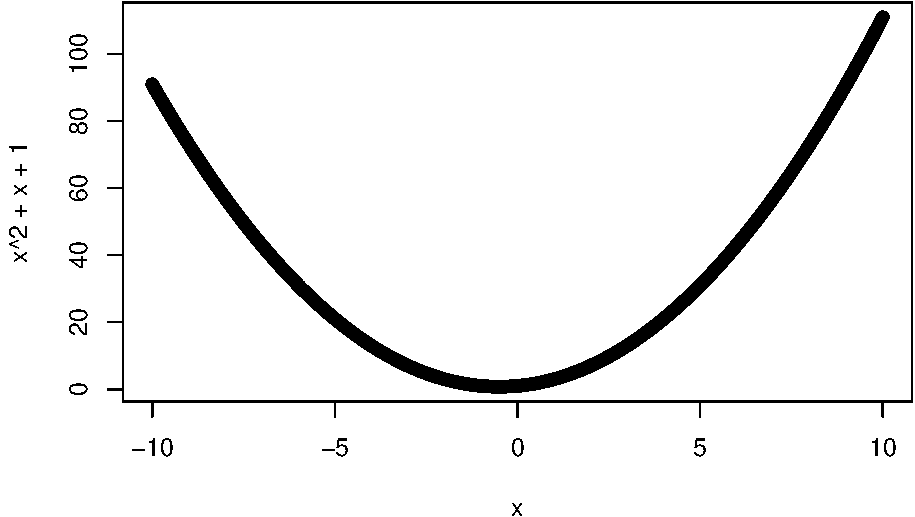
\includegraphics{informal-report_files/figure-latex/figureExample-1} \caption{figure example}\label{fig:figureExample}
\end{figure}

Figure \ref{fig:figureExample} is an example of a figure.

\newpage
\anappendix{Another appendix}

\begin{table}

\caption{\label{tab:xtable-example}Data structure for analysis}
\centering
\begin{tabular}[t]{l|r|r|r|r|r|r|r|r|r|r|r}
\hline
  & mpg & cyl & disp & hp & drat & wt & qsec & vs & am & gear & carb\\
\hline
Mazda RX4 & 21.0 & 6 & 160.0 & 110 & 3.90 & 2.620 & 16.46 & 0 & 1 & 4 & 4\\
\hline
Mazda RX4 Wag & 21.0 & 6 & 160.0 & 110 & 3.90 & 2.875 & 17.02 & 0 & 1 & 4 & 4\\
\hline
Datsun 710 & 22.8 & 4 & 108.0 & 93 & 3.85 & 2.320 & 18.61 & 1 & 1 & 4 & 1\\
\hline
Hornet 4 Drive & 21.4 & 6 & 258.0 & 110 & 3.08 & 3.215 & 19.44 & 1 & 0 & 3 & 1\\
\hline
Hornet Sportabout & 18.7 & 8 & 360.0 & 175 & 3.15 & 3.440 & 17.02 & 0 & 0 & 3 & 2\\
\hline
Valiant & 18.1 & 6 & 225.0 & 105 & 2.76 & 3.460 & 20.22 & 1 & 0 & 3 & 1\\
\hline
Duster 360 & 14.3 & 8 & 360.0 & 245 & 3.21 & 3.570 & 15.84 & 0 & 0 & 3 & 4\\
\hline
Merc 240D & 24.4 & 4 & 146.7 & 62 & 3.69 & 3.190 & 20.00 & 1 & 0 & 4 & 2\\
\hline
Merc 230 & 22.8 & 4 & 140.8 & 95 & 3.92 & 3.150 & 22.90 & 1 & 0 & 4 & 2\\
\hline
Merc 280 & 19.2 & 6 & 167.6 & 123 & 3.92 & 3.440 & 18.30 & 1 & 0 & 4 & 4\\
\hline
Merc 280C & 17.8 & 6 & 167.6 & 123 & 3.92 & 3.440 & 18.90 & 1 & 0 & 4 & 4\\
\hline
Merc 450SE & 16.4 & 8 & 275.8 & 180 & 3.07 & 4.070 & 17.40 & 0 & 0 & 3 & 3\\
\hline
Merc 450SL & 17.3 & 8 & 275.8 & 180 & 3.07 & 3.730 & 17.60 & 0 & 0 & 3 & 3\\
\hline
Merc 450SLC & 15.2 & 8 & 275.8 & 180 & 3.07 & 3.780 & 18.00 & 0 & 0 & 3 & 3\\
\hline
Cadillac Fleetwood & 10.4 & 8 & 472.0 & 205 & 2.93 & 5.250 & 17.98 & 0 & 0 & 3 & 4\\
\hline
Lincoln Continental & 10.4 & 8 & 460.0 & 215 & 3.00 & 5.424 & 17.82 & 0 & 0 & 3 & 4\\
\hline
Chrysler Imperial & 14.7 & 8 & 440.0 & 230 & 3.23 & 5.345 & 17.42 & 0 & 0 & 3 & 4\\
\hline
Fiat 128 & 32.4 & 4 & 78.7 & 66 & 4.08 & 2.200 & 19.47 & 1 & 1 & 4 & 1\\
\hline
Honda Civic & 30.4 & 4 & 75.7 & 52 & 4.93 & 1.615 & 18.52 & 1 & 1 & 4 & 2\\
\hline
Toyota Corolla & 33.9 & 4 & 71.1 & 65 & 4.22 & 1.835 & 19.90 & 1 & 1 & 4 & 1\\
\hline
Toyota Corona & 21.5 & 4 & 120.1 & 97 & 3.70 & 2.465 & 20.01 & 1 & 0 & 3 & 1\\
\hline
Dodge Challenger & 15.5 & 8 & 318.0 & 150 & 2.76 & 3.520 & 16.87 & 0 & 0 & 3 & 2\\
\hline
AMC Javelin & 15.2 & 8 & 304.0 & 150 & 3.15 & 3.435 & 17.30 & 0 & 0 & 3 & 2\\
\hline
Camaro Z28 & 13.3 & 8 & 350.0 & 245 & 3.73 & 3.840 & 15.41 & 0 & 0 & 3 & 4\\
\hline
Pontiac Firebird & 19.2 & 8 & 400.0 & 175 & 3.08 & 3.845 & 17.05 & 0 & 0 & 3 & 2\\
\hline
Fiat X1-9 & 27.3 & 4 & 79.0 & 66 & 4.08 & 1.935 & 18.90 & 1 & 1 & 4 & 1\\
\hline
Porsche 914-2 & 26.0 & 4 & 120.3 & 91 & 4.43 & 2.140 & 16.70 & 0 & 1 & 5 & 2\\
\hline
Lotus Europa & 30.4 & 4 & 95.1 & 113 & 3.77 & 1.513 & 16.90 & 1 & 1 & 5 & 2\\
\hline
Ford Pantera L & 15.8 & 8 & 351.0 & 264 & 4.22 & 3.170 & 14.50 & 0 & 1 & 5 & 4\\
\hline
Ferrari Dino & 19.7 & 6 & 145.0 & 175 & 3.62 & 2.770 & 15.50 & 0 & 1 & 5 & 6\\
\hline
Maserati Bora & 15.0 & 8 & 301.0 & 335 & 3.54 & 3.570 & 14.60 & 0 & 1 & 5 & 8\\
\hline
Volvo 142E & 21.4 & 4 & 121.0 & 109 & 4.11 & 2.780 & 18.60 & 1 & 1 & 4 & 2\\
\hline
\end{tabular}
\end{table}

Table \ref{tab:xtable-example} is an example of a table.

\pagenumbering{arabic}
\renewcommand{\thepage}{\thesection--\arabic{page}}

\appendicesendhere

\startofreferences      %%%%%%%%%%%%%%%%%%%%%%%%%%%%%%%%%%%%%%%%%%%%%%%%%%%%%%%%%%%%%%%%%%%%%%%%%



\newpage
\singlespacing 

  {\printbibheading}
  \printbibliography[heading=none]


\end{document}
